\documentclass[11pt]{article}
\usepackage[margin=1in]{geometry}
\usepackage[T1]{fontenc}
\usepackage[utf8]{inputenc}
\usepackage{lmodern}
\usepackage{microtype}
\usepackage{graphicx}
\usepackage{booktabs}
\usepackage{array}
\usepackage{longtable}
\usepackage{float}
\usepackage{hyperref}
\usepackage{xcolor}
\usepackage{caption}

\hypersetup{
  colorlinks=true,
  linkcolor=blue!50!black,
  urlcolor=blue!50!black,
  citecolor=blue!50!black
}

\graphicspath{{../publication_assets/figures/}}

\title{Algorithmic Solvability from Examples:\\A Prepublication Benchmark Analysis of Learned Generalization, Diagnostics, and Symbolic Recovery}
\author{Prepared from the DataScience workspace on 2026-03-26}
\date{}

\begin{document}
\maketitle

\begin{abstract}
We evaluate whether a task's input-output behavior provides empirical evidence that it is governed by a compact deterministic algorithm. The implemented benchmark spans two modalities: symbolic sequence tasks and mixed-type tabular classification tasks. We reran the complete current stack, including validation tests, smoke checks, baseline suites, diagnostics, and bonus symbolic recovery, and then regenerated all manuscript figures and tables from a dedicated publication-asset pipeline. Across the implemented benchmark we evaluate 30 tasks over sequence tiers \texttt{S0-S3} and classification tiers \texttt{C0-C3}. The empirical picture is sharply asymmetric. Classification is already strong: 11 of 14 classification or control tasks are labeled \texttt{MODERATE} at baseline, and diagnostics promote one task (\texttt{C1.1\_numeric\_threshold}) to \texttt{STRONG}. Sequence learning remains weak: 12 of 16 sequence or control tasks remain \texttt{NEGATIVE}, with only \texttt{S1.4\_count\_symbol} and \texttt{S2.2\_balanced\_parens} reaching \texttt{WEAK}. Diagnostics mostly reinforce, rather than overturn, the baseline picture: sample-efficiency, distractor, noise, and feature-alignment checks are broadly favorable on tested classification subsets, while \texttt{C3.1\_xor} exposes a meaningful distractor fragility. Bonus symbolic recovery is substantially stronger than learned sequence generalization, with rule extraction passing 9 of 12 tasks and DSL program search recovering 7 of 9 tasks. The evidence therefore supports a careful claim: the current benchmark already yields convincing evidence of algorithmic solvability for many implemented tabular rule tasks, but learned sequence generalization remains the main scientific bottleneck.
\end{abstract}

\section{Introduction}

Learning systems can often fit input-output mappings without demonstrating the kind of extrapolative structure that would justify calling a task ``algorithmically solved.'' This distinction matters in work on systematic generalization and neural algorithmic reasoning, where high in-distribution accuracy can coexist with poor compositional or out-of-distribution behavior \cite{lake2018scan,kim2020cogs,velickovic2022clrs}. It also matters for symbolic recovery: a task may be algorithmically well-formed and even symbolically recoverable from examples, while the learned predictor still fails to generalize broadly \cite{balog2017deepcoder}.

This paper studies that distinction on a synthetic benchmark in which every dataset is generated by a known deterministic reference procedure. The benchmark contains two tracks. The first track covers symbolic sequence transformations and sequence-derived outputs. The second covers mixed-type tabular classification tasks whose labels are produced by explicit rule-based decision procedures. The central question is not whether a model can memorize training data, but whether the pattern of success and failure across stronger evaluation regimes provides empirical evidence that the underlying mapping is algorithmically solvable from examples.

The contribution of this paper is empirical rather than architectural. We do not introduce a new learner. Instead, we present a cleaned, rerun, and publication-audited analysis of the currently implemented benchmark. Three conclusions emerge. First, the tabular classification track already provides substantial evidence of algorithmic solvability on many deterministic rule tasks. Second, the symbolic sequence track remains weak under the current learned model family. Third, bonus symbolic recovery succeeds much more often than learned sequence generalization, suggesting that the benchmark design is ahead of the present sequence learners rather than the reverse.

\section{Benchmark and Evaluation Protocol}

\subsection{Implemented scope}

The current benchmark implements 30 tasks across eight tiers. Table~\ref{tab:inventory} summarizes the executed scope.

\begin{table}[H]
\centering
\caption{Implemented benchmark inventory.}
\label{tab:inventory}
\begin{tabular}{lcc}
\toprule
Track & Implemented tiers & Tasks \\
\midrule
Sequence & \texttt{S0}, \texttt{S1}, \texttt{S2}, \texttt{S3} & 16 \\
Classification & \texttt{C0}, \texttt{C1}, \texttt{C2}, \texttt{C3} & 14 \\
\bottomrule
\end{tabular}
\end{table}

The benchmark should therefore be interpreted as an \texttt{S0-S3} and \texttt{C0-C3} study. The broader aspirational tier system in the design notes is useful for roadmap purposes, but the evidence in this paper is limited to the implemented tiers.

\subsection{Task generation and splits}

All tasks are synthetic and deterministic. Sequence tasks operate on variable-length symbolic inputs. Classification tasks operate on fixed-width mixed numerical and categorical feature vectors. In each case, the label or output is produced by a reference algorithm known to the benchmark. This lets us generate unlimited data, evaluate exact correctness, and construct targeted split families that test more than IID interpolation.

The executed suites use IID and out-of-distribution regimes appropriate to each modality. For sequence tasks, the current runs include IID, length extrapolation, and value extrapolation. For classification tasks, the current runs include IID, value extrapolation, and noise-oriented robustness splits, with additional targeted diagnostics for distractors, feature salience, and sample efficiency.

\subsection{Evidence labels}

Each task receives a composite solvability score and a categorical evidence label. The label semantics follow the benchmark design:

\begin{itemize}
  \item \textbf{STRONG}: criteria 1--5 are met, plus at least two stronger diagnostic criteria;
  \item \textbf{MODERATE}: criteria 1--5 are met;
  \item \textbf{WEAK}: only the basic IID criterion is clearly met;
  \item \textbf{NEGATIVE}: tested models fail to show meaningful solvability evidence;
  \item \textbf{INCONCLUSIVE}: the evidence is mixed or confounded.
\end{itemize}

This matters because the paper's claims rest on evidence labels, not on isolated accuracy values.

\section{Experimental Setup}

\subsection{Model families executed}

The present sequence suites use the model families logged in the experiment configs: \texttt{majority\_class}, \texttt{sequence\_baseline}, \texttt{mlp}, and \texttt{lstm}. The present classification suites use \texttt{majority\_class}, \texttt{logistic\_regression}, \texttt{decision\_tree}, \texttt{random\_forest}, \texttt{gradient\_boosted\_trees}, and \texttt{mlp}. These are the actual executed model families in the rerun reported here; we intentionally avoid describing broader aspirational model families that were not part of the current artifact set.

\subsection{Validation and rerun status}

Before regenerating figures and tables, we reran the full validation and experiment stack from the checked-in virtual environment:

\begin{itemize}
  \item \texttt{python -m pytest -q}
  \item \texttt{python main.py smoke}
  \item \texttt{python main.py sequence}
  \item \texttt{python main.py classification}
  \item \texttt{python main.py diagnostic}
  \item \texttt{python main.py bonus}
\end{itemize}

The test suite passed with 460 tests and 17 warnings. The warnings were optimizer and high-cardinality warnings in the training stack, not correctness failures. The full experiment rerun completed successfully. A dedicated publication-asset script then regenerated all tables and figures into \texttt{output/publication\_assets/}. We visually reviewed the figure outputs before finalizing the manuscript.

\section{Baseline Results}

Track-level baseline summaries are shown in Table~\ref{tab:baseline-summary}, and the label distribution is shown in Figure~\ref{fig:baseline-dist}.

\begin{table}[H]
\centering
\caption{Baseline summary by track.}
\label{tab:baseline-summary}
\begin{tabular}{lrrrrrr}
\toprule
Track & Tasks & Mean score & Mean best IID & Mean best OOD & Negative & Moderate \\
\midrule
Sequence & 16 & 0.3359 & 0.3195 & 0.2135 & 12 & 0 \\
Classification & 14 & 0.6753 & 0.9355 & 0.9702 & 1 & 11 \\
\bottomrule
\end{tabular}
\end{table}

\begin{figure}[H]
\centering
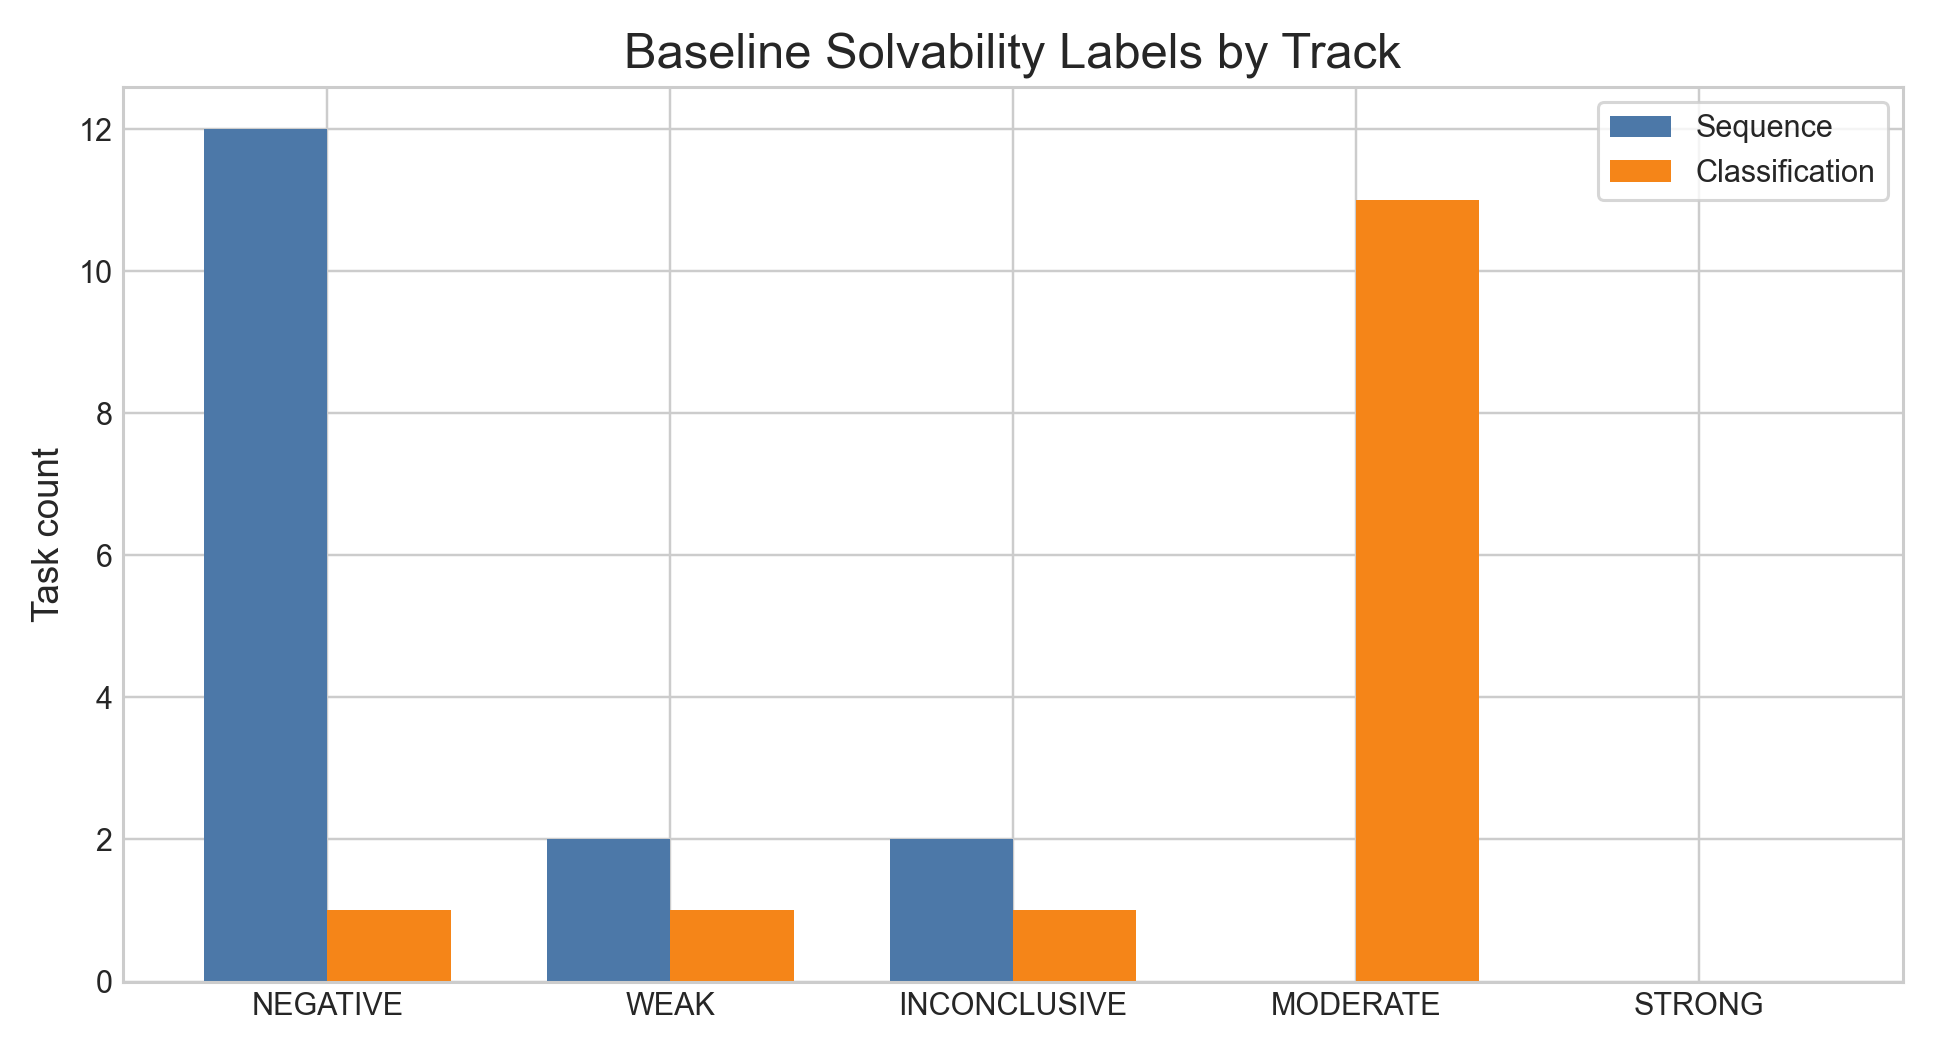
\includegraphics[width=0.84\textwidth]{baseline_verdict_distribution.png}
\caption{Baseline solvability labels by track. The classification track concentrates mass in \texttt{MODERATE}, whereas the sequence track remains dominated by \texttt{NEGATIVE}.}
\label{fig:baseline-dist}
\end{figure}

The broad result is a modal asymmetry. The classification track already supports the core benchmark claim on most implemented tasks. The sequence track does not. Figure~\ref{fig:iid-ood} makes that split especially clear at task level.

\begin{figure}[H]
\centering
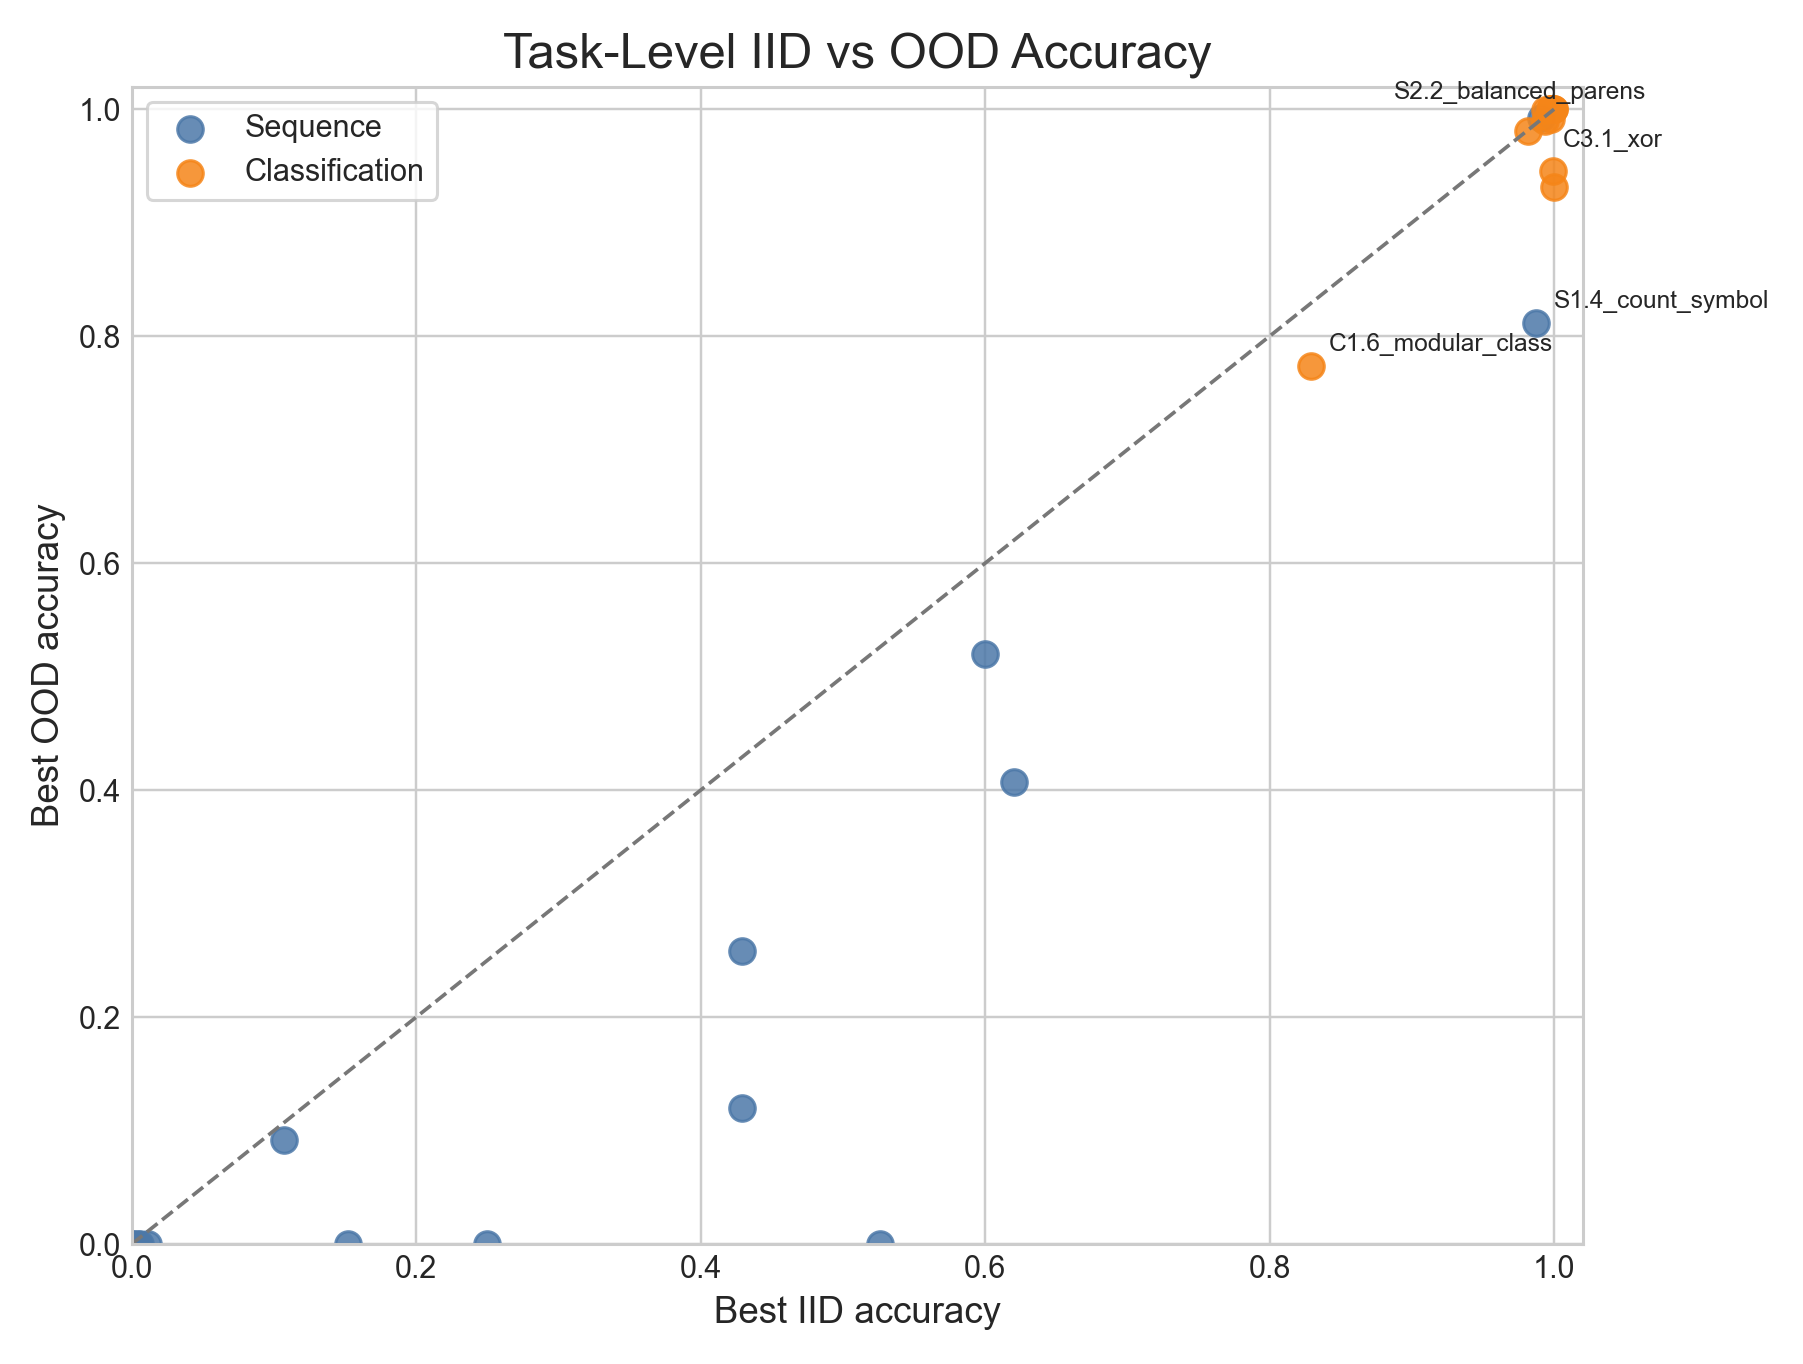
\includegraphics[width=0.80\textwidth]{iid_vs_ood_accuracy.png}
\caption{Task-level IID versus OOD accuracy. Classification tasks cluster near the upper-right corner, while sequence tasks occupy a much weaker region with only a few exceptions.}
\label{fig:iid-ood}
\end{figure}

\subsection{Classification}

The classification results are strong but not uniform. Eleven of fourteen classification or control tasks achieve \texttt{MODERATE} evidence at baseline. The strongest baseline tasks include \texttt{C2.3\_nested\_if\_else}, \texttt{C1.2\_range\_binning}, \texttt{C3.3\_rank\_based}, \texttt{C1.1\_numeric\_threshold}, and \texttt{C2.6\_categorical\_gate}. These tasks combine high IID performance with strong out-of-distribution behavior under the currently implemented split families.

The classification results are not trivial or uniformly easy. The control task \texttt{C0.1\_random\_class} remains \texttt{NEGATIVE}. The modular arithmetic task \texttt{C1.6\_modular\_class} remains \texttt{INCONCLUSIVE}. The conjunction task \texttt{C2.1\_and\_rule} reaches only \texttt{WEAK}, despite near-perfect raw accuracy, because it does not satisfy the full evidence bundle needed for a stronger label. These cases are important because they show that the benchmark is not merely rewarding high accuracy with optimistic solvability labels.

\subsection{Sequence}

The sequence story is much weaker. Twelve of sixteen sequence or control tasks remain \texttt{NEGATIVE}, and no sequence task reaches \texttt{MODERATE}. Only \texttt{S1.4\_count\_symbol} and \texttt{S2.2\_balanced\_parens} reach \texttt{WEAK}. A few other tasks such as \texttt{S1.5\_parity} and \texttt{S1.8\_extrema} show partial signal, but not enough to support a stronger claim.

This weak result should not be hidden by the few successful points in Figure~\ref{fig:iid-ood}. The correct reading is that current learned sequence models extract some algorithmic signal, but they do not yet provide broad evidence of learned algorithmic solvability across the implemented symbolic benchmark.

\section{Diagnostic Results}

The diagnostic suite asks whether the favorable baseline tasks still behave algorithmically under more targeted tests. Table~\ref{tab:diagnostics} summarizes the diagnostic outcomes, and Figure~\ref{fig:diag-matrix} visualizes pass, fail, and non-evaluated cells.

\begin{table}[H]
\centering
\caption{Diagnostic overview.}
\label{tab:diagnostics}
\begin{tabular}{lrrrc}
\toprule
Diagnostic & Unit & Evaluated & Positive outcomes & Rate \\
\midrule
\texttt{EXP-D1} sample efficiency & tasks & 8 & 6 & 0.75 \\
\texttt{EXP-D2} distractor robustness & tasks & 5 & 4 & 0.80 \\
\texttt{EXP-D3} noise robustness & tasks & 4 & 4 & 1.00 \\
\texttt{EXP-D4} feature alignment & task-model pairs & 9 & 9 & 1.00 \\
\texttt{EXP-D5} label changes & tasks & 30 & 1 & 0.0333 \\
\bottomrule
\end{tabular}
\end{table}

\begin{figure}[H]
\centering
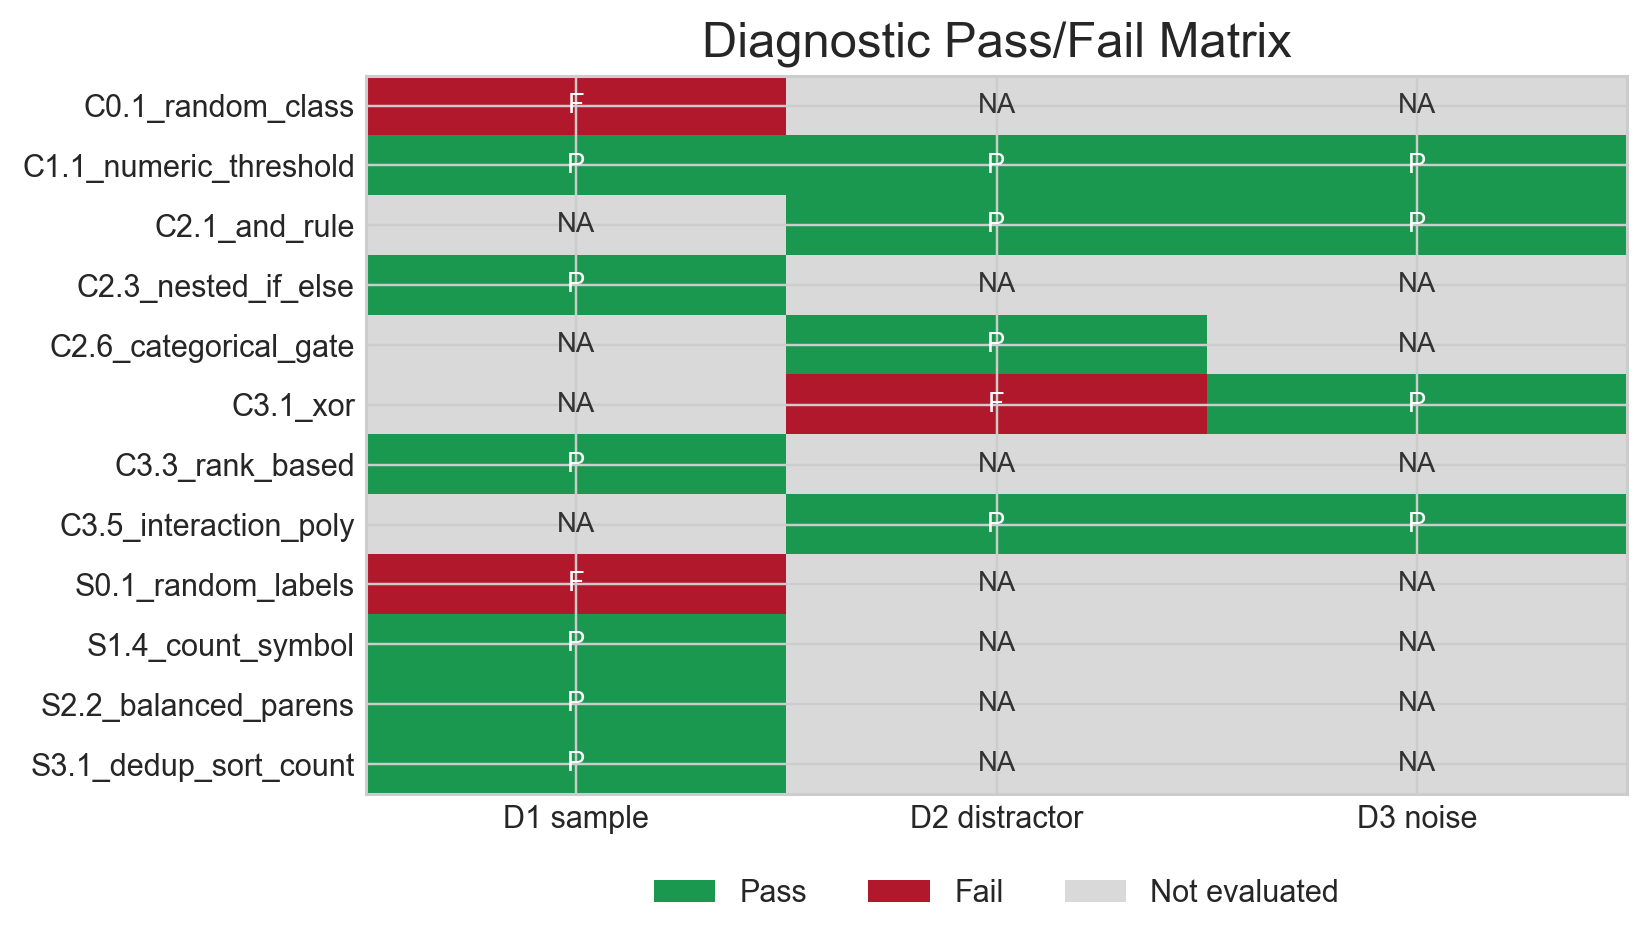
\includegraphics[width=0.88\textwidth]{diagnostic_matrix.png}
\caption{Diagnostic pass and fail matrix. Diagnostics are mostly favorable on the tested classification subset, while controls behave as intended and many cells remain intentionally unevaluated rather than implicitly passed.}
\label{fig:diag-matrix}
\end{figure}

The most important message is that diagnostics mostly reinforce the classification results rather than overturning them. Sample efficiency separates intended algorithmic tasks from controls. Distractor robustness is strong on most tested classification tasks. Noise robustness is uniformly strong on its tested subset. Feature-importance alignment is perfect on the tested task-model pairs.

At the same time, diagnostics expose a nontrivial weakness: \texttt{C3.1\_xor} fails distractor robustness. This is exactly the kind of result the benchmark should reveal. High baseline accuracy alone is not enough; a model can still be brittle under irrelevant-feature intervention.

Diagnostics do not materially change the benchmark-wide conclusion. Calibration upgrades only one task:

\begin{itemize}
  \item \texttt{C1.1\_numeric\_threshold}: \texttt{MODERATE} $\rightarrow$ \texttt{STRONG}
\end{itemize}

All sixteen sequence tasks remain in their original label categories after calibration. Thirteen of fourteen classification tasks also remain in their original category. The calibration stage is therefore confirmatory rather than transformative.

\section{Bonus Symbolic Recovery}

The bonus stage asks whether tasks that appear algorithmically structured can be recovered more directly by symbolic procedures. Table~\ref{tab:bonus} and Figure~\ref{fig:bonus} summarize the results.

\begin{table}[H]
\centering
\caption{Bonus symbolic recovery summary.}
\label{tab:bonus}
\begin{tabular}{lrrr}
\toprule
Experiment & Tasks evaluated & Tasks passing & Pass rate \\
\midrule
\texttt{EXP-B1} rule extraction & 12 & 9 & 0.7500 \\
\texttt{EXP-B2} program search & 9 & 7 & 0.7778 \\
\bottomrule
\end{tabular}
\end{table}

\begin{figure}[H]
\centering
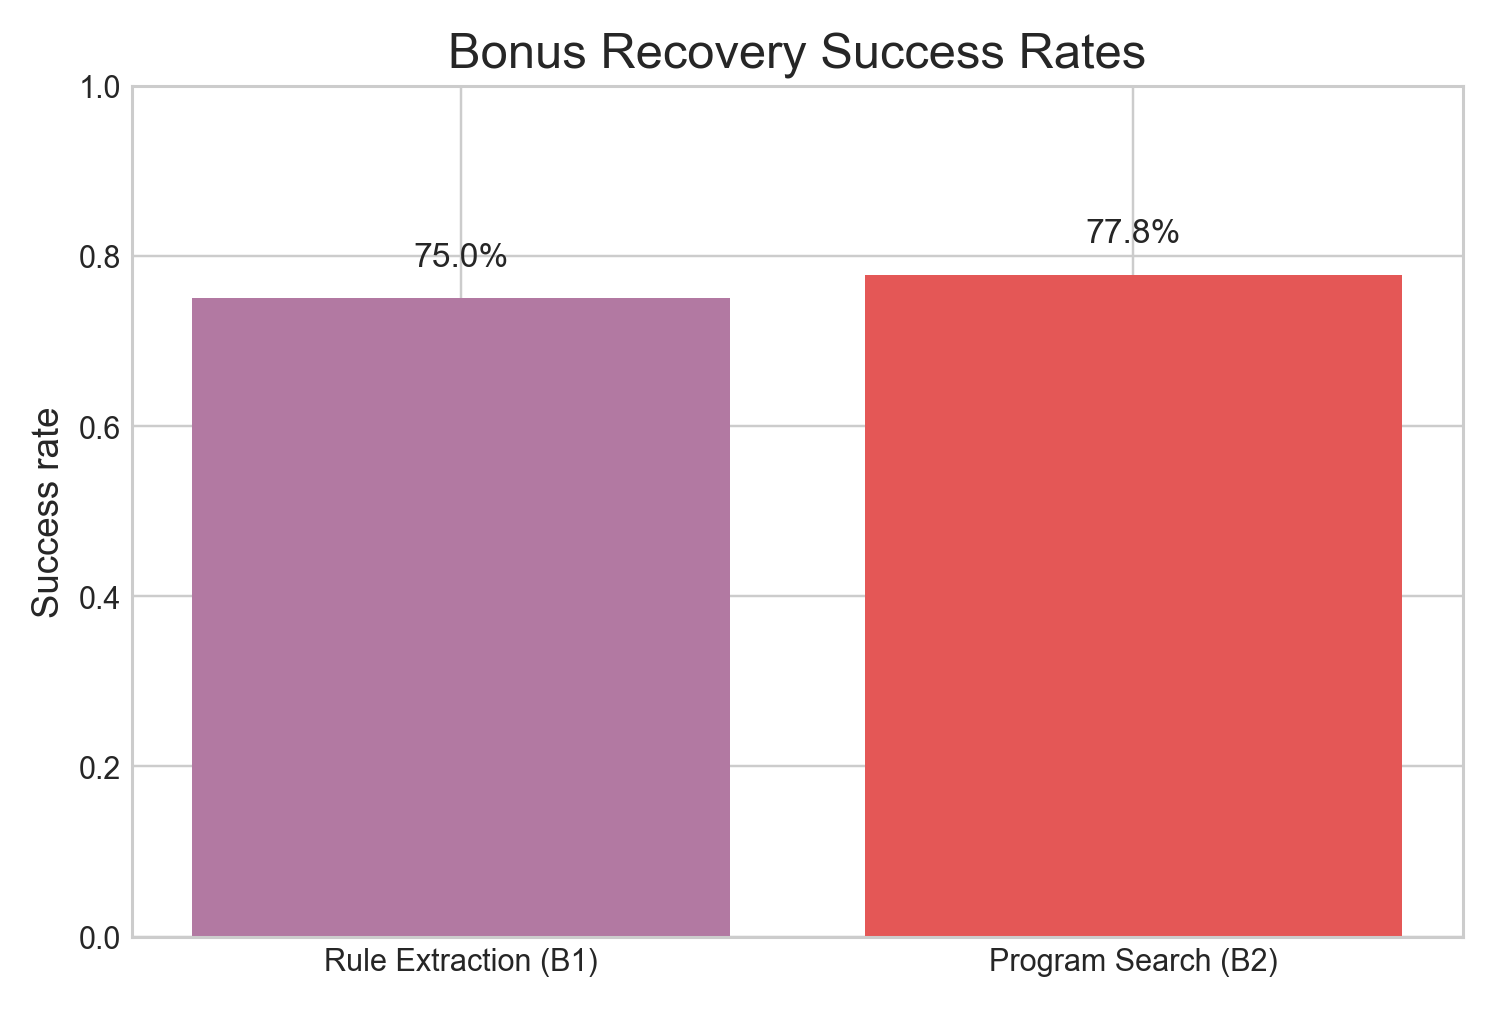
\includegraphics[width=0.64\textwidth]{bonus_success_rates.png}
\caption{Bonus symbolic recovery success rates. Symbolic recovery succeeds much more often than learned sequence generalization, especially on the program-search side.}
\label{fig:bonus}
\end{figure}

These results are central to the interpretation of the weak sequence track. If both learned models and symbolic search were failing, the benchmark tasks themselves would be suspect. That is not what we observe. Instead, symbolic recovery succeeds on most searched classification and sequence tasks. The most plausible interpretation is that the sequence benchmarks are algorithmically coherent, but the present learned sequence models are not yet strong enough to extract the underlying procedure reliably.

\section{Threats to Validity and Remaining Limitations}

Several limitations should be stated directly.

\paragraph{Implemented scope.}
The evidence in this paper covers only the implemented tiers \texttt{S0-S3} and \texttt{C0-C3}. It should not be generalized to the full aspirational benchmark roadmap.

\paragraph{Diagnostic coverage.}
The diagnostic suite evaluates targeted subsets. A missing cell in Figure~\ref{fig:diag-matrix} means ``not evaluated,'' not ``implicitly passed.'' Reviewers should therefore read the diagnostic evidence as focused support rather than exhaustive coverage.

\paragraph{Training-stack warnings.}
The rerun is correctness-clean, but not optimization-clean. MLP and logistic-regression convergence warnings remain in the stack and should be treated as technical debt rather than ignored.

\paragraph{Runtime logging.}
Not all experiment summaries log runtime. The fresh rerun completed successfully, and shell-measured wall-clock times indicate that the full experiment stack now runs in about 16 minutes, but several diagnostic and bonus summaries do not yet expose recoverable runtime in their own artifacts.

\paragraph{Sequence conclusions are model-family dependent.}
The weak sequence result is a statement about the currently executed model family in this repository. It is not evidence that the underlying sequence tasks are unsolvable by stronger or differently biased architectures.

\section{Reproducibility}

The paper was assembled from a dedicated publication asset bundle regenerated after the fresh rerun:

\begin{itemize}
  \item derived tables and summaries: \texttt{output/publication\_assets/data/}
  \item publication figures: \texttt{output/publication\_assets/figures/}
  \item completeness checklist: \texttt{output/publication\_assets/data/publication\_checklist.md}
\end{itemize}

This separation is deliberate. The manuscript is not built from ad hoc notes or copied terminal output. Instead, the figures and tables in the paper are downstream products of the rerun artifacts. That workflow materially reduces the risk of narrative drift between the result files and the paper text.

\section{Conclusion}

The current benchmark now supports a paper with a precise and defensible claim. On the implemented tabular classification tasks, standard learning systems already provide broad evidence of algorithmic solvability from examples. On the implemented symbolic sequence tasks, they do not. Diagnostics largely strengthen the positive classification story, while bonus symbolic recovery suggests that weak sequence performance is more likely a limitation of the present learners than of the benchmark design.

The right conclusion is therefore neither triumphalist nor pessimistic. The benchmark is already scientifically useful. It can separate strong from weak task families, surface nontrivial failure modes such as distractor fragility, and distinguish learned generalization from symbolic recoverability. The next stage of work should focus on improving sequence representations and inductive biases while preserving the now-stable experimental and reporting pipeline.

\appendix

\section{Top Calibrated Tasks}

Table~\ref{tab:top-calibrated} lists the highest-scoring calibrated tasks.

\begin{longtable}{llrr}
\caption{Top calibrated tasks.}
\label{tab:top-calibrated}\\
\toprule
Task & Final label & Calibrated score & Track \\
\midrule
\endfirsthead
\toprule
Task & Final label & Calibrated score & Track \\
\midrule
\endhead
\texttt{C1.1\_numeric\_threshold} & \texttt{STRONG} & 0.9291 & classification \\
\texttt{C2.3\_nested\_if\_else} & \texttt{MODERATE} & 0.8535 & classification \\
\texttt{C3.3\_rank\_based} & \texttt{MODERATE} & 0.8466 & classification \\
\texttt{C2.6\_categorical\_gate} & \texttt{MODERATE} & 0.8266 & classification \\
\texttt{C3.5\_interaction\_poly} & \texttt{MODERATE} & 0.8001 & classification \\
\texttt{C3.1\_xor} & \texttt{MODERATE} & 0.7785 & classification \\
\texttt{C2.1\_and\_rule} & \texttt{WEAK} & 0.7700 & classification \\
\texttt{C1.2\_range\_binning} & \texttt{MODERATE} & 0.7480 & classification \\
\texttt{S2.2\_balanced\_parens} & \texttt{WEAK} & 0.7465 & sequence \\
\texttt{C1.5\_numeric\_comparison} & \texttt{MODERATE} & 0.7242 & classification \\
\bottomrule
\end{longtable}

\begin{figure}[H]
\centering
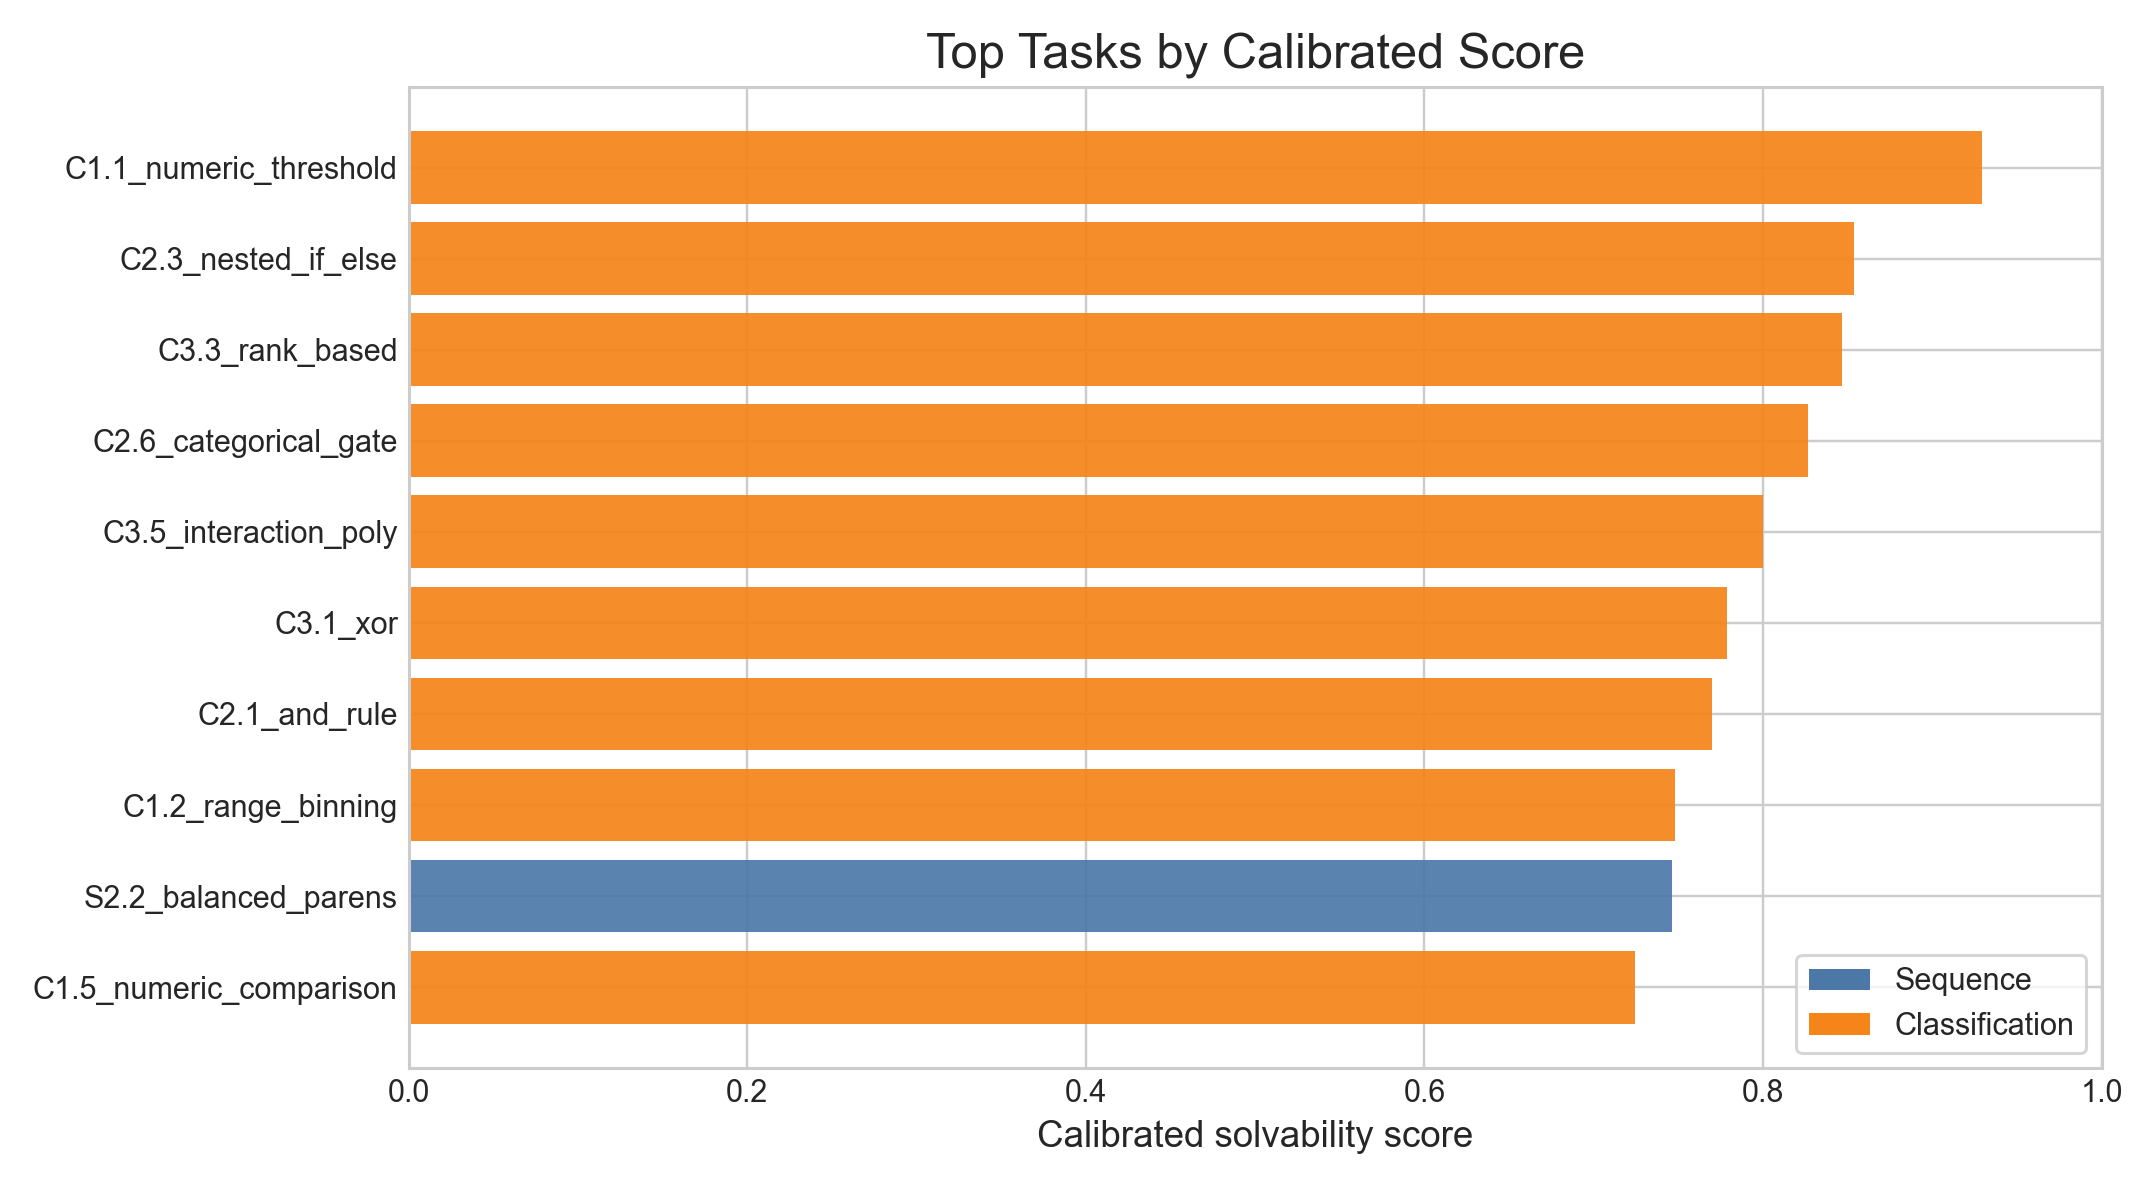
\includegraphics[width=0.86\textwidth]{top_calibrated_scores.png}
\caption{Appendix view of the highest calibrated solvability scores. The top of the ranking is dominated by classification tasks, with \texttt{S2.2\_balanced\_parens} as the only sequence task in the top ten.}
\label{fig:top-calibrated}
\end{figure}

\begin{thebibliography}{9}

\bibitem{lake2018scan}
Brenden M. Lake and Marco Baroni.
\newblock Generalization without systematicity: On the compositional skills of sequence-to-sequence recurrent networks.
\newblock In \emph{Proceedings of the 35th International Conference on Machine Learning}, 2018.
\newblock Available at \href{https://proceedings.mlr.press/v80/lake18a.html}{proceedings.mlr.press/v80/lake18a.html}.

\bibitem{kim2020cogs}
Najoung Kim and Tal Linzen.
\newblock {COGS}: A compositional generalization challenge based on semantic interpretation.
\newblock In \emph{Proceedings of the 2020 Conference on Empirical Methods in Natural Language Processing (EMNLP)}, pages 9087--9105, 2020.
\newblock Available at \href{https://aclanthology.org/2020.emnlp-main.731/}{aclanthology.org/2020.emnlp-main.731/}.

\bibitem{balog2017deepcoder}
Matej Balog, Alexander L. Gaunt, Marc Brockschmidt, Sebastian Nowozin, and Daniel Tarlow.
\newblock DeepCoder: Learning to write programs.
\newblock In \emph{Proceedings of the International Conference on Learning Representations (ICLR)}, 2017.
\newblock Available at \href{https://openreview.net/pdf?id=rkE3y85ee}{openreview.net/pdf?id=rkE3y85ee}.

\bibitem{velickovic2022clrs}
Petar Veli\v{c}kovi\'{c}, Adri\`{a} Puigdom\`{e}nech Badia, David Budden, Razvan Pascanu, Andrea Banino, Misha Dashevskiy, Raia Hadsell, and Charles Blundell.
\newblock The {CLRS} algorithmic reasoning benchmark.
\newblock arXiv preprint arXiv:2205.15659, 2022.
\newblock Available at \href{https://arxiv.org/abs/2205.15659}{arxiv.org/abs/2205.15659}.

\end{thebibliography}

\end{document}
